\documentclass[a4paper,10pt]{article}

\setlength{\textwidth}{7in}
\setlength{\textheight}{9in}
\setlength{\oddsidemargin}{-0.35in}
\setlength{\topmargin}{-0.5in}

\usepackage{multicol}       %% Omogoči dvostolpično besedilo
\usepackage[affil-it]{authblk}   %%Omogoči označevanje avtorjev. Opcija affil-it naredi affiliation italic
\usepackage[slovene, english]{babel}		%% Izbrana slovenski in angleški jezik za deljenje besed		


\usepackage[utf8]{inputenc} %% Delujejo tudi šumniki s tisto enkripcijo, s katero vnašamo tekst

\usepackage[it]{caption}
\setlength{\captionmargin}{10pt}
\setlength{\abovecaptionskip}{0pt}
\setlength{\belowcaptionskip}{10pt}

\usepackage{amsmath}
\usepackage{graphicx}
\usepackage{float}
\usepackage{epstopdf}
\usepackage{amsmath}
\usepackage{amsfonts}
\usepackage{amssymb}
\usepackage{array}
\usepackage[numbers,square,sort&compress]{natbib}






\title{\bf{Analiza izkoristkov termoelektrarn}}


\author{Mitja Alič}
%\author[2]{Drugi Avtor}
%\author[1,2]{Tretji Vodilni Avtor} %\thanks{Ime organizacije \\ naslov organizacije \\ zip Mesto \\ Država \\ avtor@naslov.com}}
\affil{Fakulteta za elektrotehniko, Univeraza v Ljubljani}
%\affil[2]{Ime in naslov druge organizacije}
\renewcommand\Authands{ in }
\date{\vspace{-3ex} mitja1357@gmail.com}
%\date{avtor@naslov.com}
\begin{document}
\maketitle
%Slovenski povzetek
\noindent
\textbf{\textit{Povzetek:}} {\it \textbf{IZHODIŠČA}. Termoelektrarna proizvaja elektriko na podlagi krožnega procesa. Sestavljena je iz več delov, vendar se v vsakem pojavljajo izgube, ki vplivajo na skupni izkoristek termoelektrarne. Namen naše študije je bil analizirati dele termoelektrarne, izgube in kako te vplivajo na skupni izkoristek procesa.\\
	\textbf{METODE}. Pregledali smo strokovno literaturo, ki je ustrezala naši študiji, in zbrali ključne podatke.\\
\textbf{REZULTATI}. Rezultati kažejo, da na skupni izkoristek najbolj vpliva izkoristek krožnega procesa. Ostali deli termoelektrarne so primerno izkoriščeni.\\
	\textbf{ZAKLJUČEK}. Za izboljšanje skupnega izkoristka se je potrebno posvetiti krožnemu procesu.
}
\\
\noindent	
\textbf{\textit{Klju\v cne besede:}} {\it krožni proces; anergija; eksergija; turbina; generator;}
%Angleški naslov in povzetek
\selectlanguage{english}
\begin{center}
	\subsection*{ \bf Analaysis efficiency of thermal power plants} 
\end{center}
\noindent
\textbf{\textit{Abstract:}} {\it \textbf{BACKGROUND}. Thermal power plant uses the principle of the thermodynamic cycle to generate electricity. The system electricity production consists of several parts. Losses occur in every part of the production cycle and have an impact on the overall efficiency of thermal power plants. The aim of our study was to explore parts of the thermal power plant, to define losses and to describe how these losses affect the overall efficiency of the system. \\
	\textbf{METHODS}. A systematic search of bibliographic databases was performed. Crucial pieces of information were collected in this document. \\
	\textbf{RESULTS}. The results show that the overall efficiency is most affected by the efficiency of the thermodynamic cycle. Other parts of the thermal power plant are optimized. \\
	\textbf{CONCLUSION}. To improve the overall efficiency, one should improve the efficiency of the thermodynamic cycle.
}
\\
\noindent	
\textbf{\textit{Keywords:}} {\it thermodynamic cycle; anergy; exergy; turbine; generator;}
\\
\selectlanguage{slovene}
\begin{multicols}{2}
\section{Uvod}
Največ električne energije na svetu proizvedejo termoelektrarne (TE). Glede na globalne trende, se želi čim manj onesnaževati naš planet in procese čim bolj izkoristiti. S tem delom želim predstaviti procese TE, ki so del proizvodnje električne energije. Opisal bom pojavljanje izgub in kako te vplivajo na skupni izkoristek TE.
\section{Izkoristki posameznih elementov termoelektrarne}
Proces proizvodnje električne energije v TE je razdeljen na več delov. Za višji izkoristek TE, je potreben višji izkoristek posameznega dela. V posameznem podpoglavju bom opisal dele podrobneje.
\subsection{Kro"zni proces}
Vsak proces, ki ob pretvarjanju energije vrne sistem v začetno stanje, imenujemo krožni proces (slika \ref{TS}).
\begin{minipage}[H!]{\linewidth}
	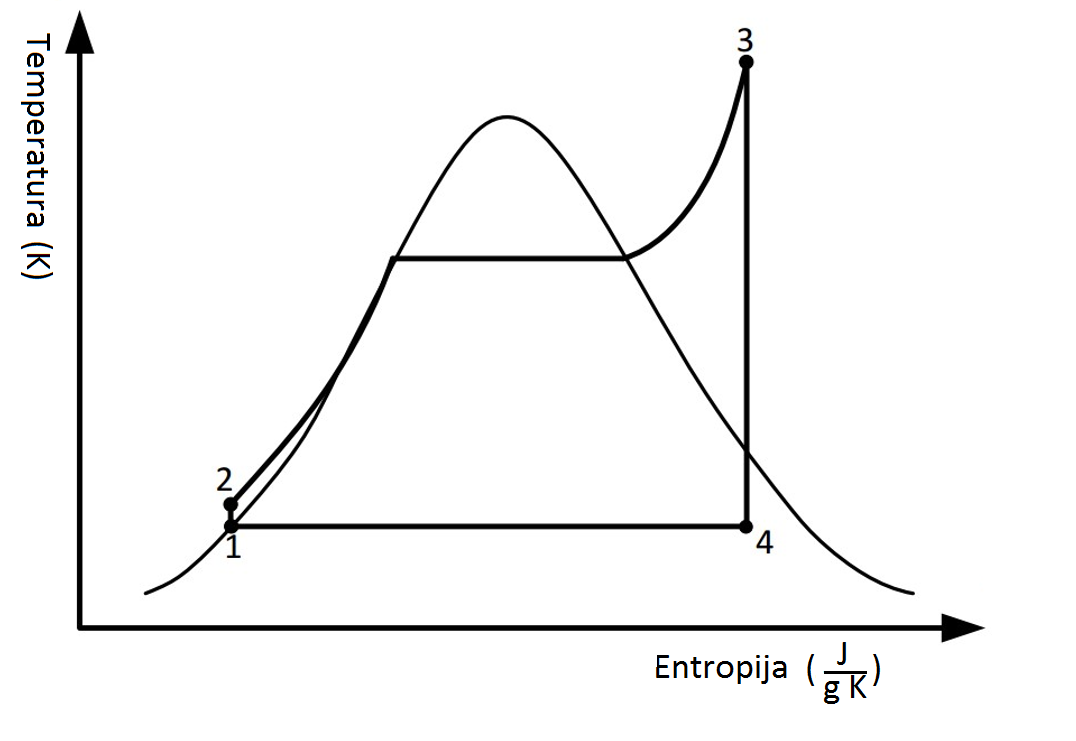
\includegraphics[width=0.85\columnwidth]{Untitled.png}
	\captionof{figure}{Grafikon parnega krožnega procesa \citep{Gasperic}}
	\label{TS}
\end{minipage}
 Vsaki točki pripada vrednost tlaka, temperature, entalpije\footnote{Entalpija je termodinamska spremenljivka, definirana kot vsota notranje energije ter produkta tlaka in volumna snovi \citep{Wiki}} in entropije. Izkoristek $\eta_{kp}$ po sliki \ref{TS} je
\begin{equation}
	\eta_{kp}=\frac{h_3-h_4-(h_2-h_1 )}{h_3-h_2 }.
\end{equation}
Razlika entalpij $h_3-h_4$ med točkama 3 in 4 predstavlja sproščeno entalpijo. Entalpija $h_2-h_1$ se porablja za spremembo nivoja tlaka iz točke 1 v točko 2. Entalpija $h_3-h_2$ predstavlja vloženo entalpijo v segrevanje vode.
\subsection{Napajalna črpalka}
Črpalke v krožnem procesu uporabljamo za:
\begin{itemize}
	\item napajanje parnega kotla
	\item črpanje kondenzata iz kondenzatorja
	\item črpanje hladilne vode
\end{itemize}		
S slike \ref{TS} vidimo delovanje napajalne črpalke med točko 1 in 2. Črpalko sestavljati elektromotor in turbina. Izkoristek je odvisen od izgub v pogonskem motorju in izgub v turbini.
Izkoristek črpalke $\eta_{"crp}$  je
\begin{equation}
	\eta_{"crp}=1-\frac{P_{it}+P_{im}}{P_{prej}}
\end{equation}
kjer $P_{it}$ predstavlja izgube na turbini, $P_{im}$ izgube v elektromotorju in $P_{prej}$ prejeto električno moč.
\begin{minipage}{\linewidth}
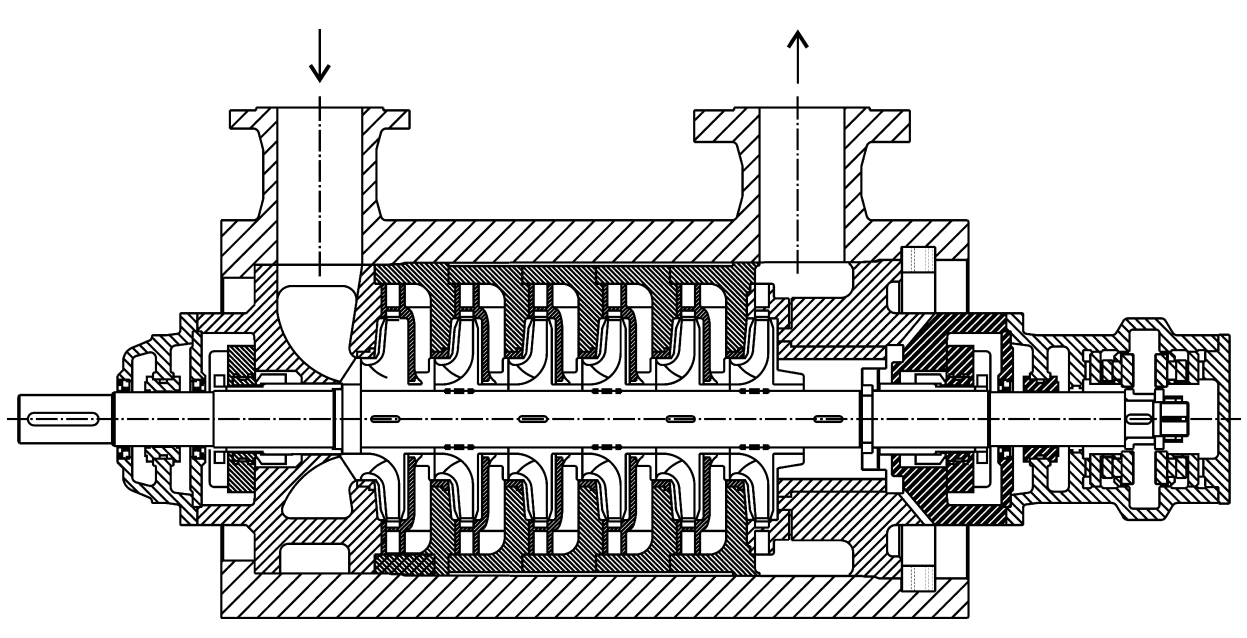
\includegraphics[width=0.95\columnwidth]{Kotlovska_crpalka.png}
\captionof{figure}{Turbina napajalne kotlovske črpalke \citep{Orel}}
\label{crp}
\end{minipage}
\subsection{Kotel}
Naloga kotla je, da toploto zgorelega goriva dovede vodi in pari.

Vsaka snov (razen izgubna toplota) ima svojo maso $m$, entalpijo $h$ in temperaturo $T$. V kotlu ni transformacije v mehansko energijo, zato je dovedena toplota enaka odvedeni. Po sliki \ref{kot1} se enačba \ref{eq1} glasi
\begin{equation}
	\begin{split}
		m_g h_g (T_1 )+ m_z h_z (T_1 )+ m_v h_v (T_2 )= \\
		= m_p h_p (T_3) + m_plini h_plini (T_plini) + Q_odv
	\end{split}
	\label{eq1}
\end{equation}
kjer $m_g h_g (T_1 )$ predstavlja energijo goriva pri temperaturi $T_1$, $m_z h_z (T_1 )$ energijo zraka pri temperaturi $T_1$, $m_v h_v (T_2 )$ energijo napajalne vode pri temperaturi $T_2$, $m_p h_p (T_3)$ energijo pare pri temperaturi $T_3$,$ m_plini h_plini (T_plini )$ energijo plinov pri temperaturi $T_{plini}$ in $Q_odv$ izgubljeno energijo.
\begin{minipage}{\linewidth}
	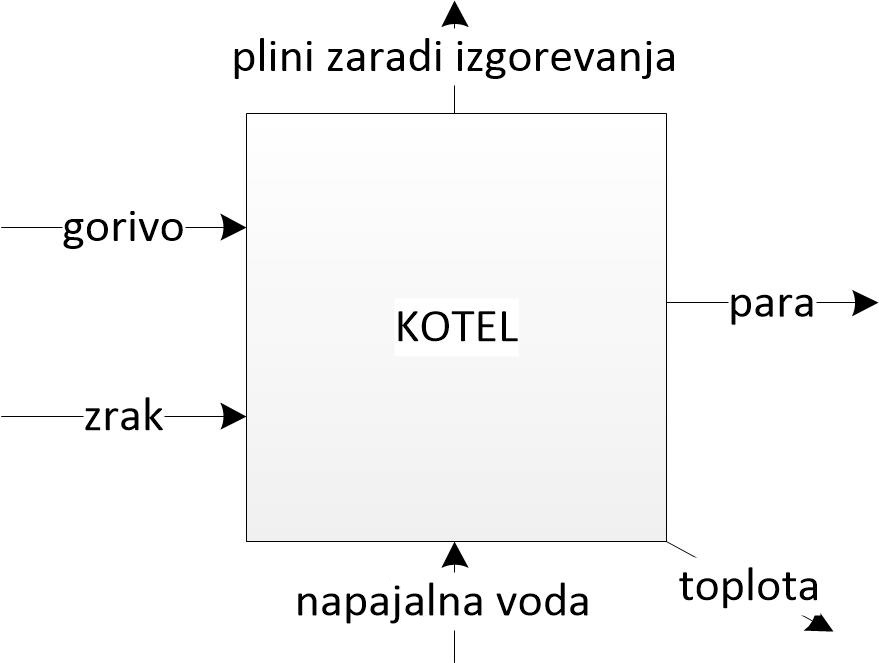
\includegraphics[width=0.95\columnwidth]{kotel.jpg}
	\captionof{figure}{Shema kotla \citep{Orel}}
	\label{kot1}
\end{minipage}
Energija dovedena z gorivom je:
\begin{equation}
	m_g h_i  = m_g h_g (T_1) + m_z h_z (T_1) - m_plini h_plini (T_1)
\end{equation}
Upoštevajmo, enakost mas vode in pare.
\begin{equation}
	\begin{split}
		m_g h_i= m_p (h_p-h_v)+m_plini (h_{plini} (T_{plini})\\-h_{plini} (T_1))+Q_{odv}
	\end{split}
\end{equation}
$h_p-h_v$ predstavlja razliko entalpij med točko 2 in točko 3. Koristna toplota je samo prvi člen in izkoristek kotla $\eta_k$ definiramo:
\begin{equation}
	\eta_k=\frac{m_p(h_3-h_2)}{m_gh_i}
\end{equation}
Za boljši izkoristek, moramo izhodno temperaturo plinov čim bolj ohladiti (s tem zmanjšamo entalpijo). Ne smemo pa je znižati pod temperaturo kondenzacije, saj bi žveplov dioksid z vodo tvoril žvepleno kislino, ki povzroča korozijo.

Iz energijskega izkoristka ne dobimo podatka o popolnosti transformacije energije. Po drugem zakonu termodinamike določimo eksergijski izkoristek kotla. Eksergija je energija, ki se lahko pri dani okolico v celoti pretvori v drugo obliko energije. Anergija je energija, ki se ne da pretvoriti v eksergijo.
Vsaka energija W je sestavljena iz anergije B  in eksergije E.\citep{Orel}
\begin{equation}
	W=B+E
\end{equation}
Po sliki \ref{kot1} napišimo enačbo eksergije
\begin{equation}
	m_g e_g+m_z e_z+m_v e_2=m_p e_3+m_plini e_plini+E_{odv},
\end{equation}
kjer $e_g$predstavlja eksergijo goriva, $e_z$eksergijo zraka, $e_2$ eksergijo napajalne vode, $e_3$ eksergijo pare, $e_{plini}$ eksergijo plinov in $E_{odv}$ izgubno eksergijo. Ker ima zrak, dovajan v kotel, temperaturo okolice, nima eksergije ($e_z=~0\frac{\mathrm{J}}{\mathrm{g}}$). Eksergije plinov na izhodu kotla ne uporabimo, saj se plini mešajo z okoliškim zrakom. Ekserzijski izkoristek $\xi_k$ je
\begin{equation}
	\xi_k=\frac{m_p(e_3-e_2)}{m_ge_g}.
\end{equation}
Iz energijskega izkoristka izrazimo razmerja mas, vstavimo v zgornjo enačbo in dobimo
\begin{equation}
	\xi_k=\frac{h_i}{e_g}\eta_k\frac{e_3-e_2}{h_3-h_2}
\label{eq10}
\end{equation}
Razliko eksergij je mogoče izračunati po enačbi
\begin{equation}
	e_3-e_2=h_3-h_2-T_3 (s_3-s_2),
\end{equation}
kjer predstavlja $s_3-s_2$ razliko entropij s slike \ref{TS} med točko 2 in 3. Vstavimo v enačbo \ref{eq10} in dobimo
\begin{equation}
	\xi_k=\frac{h_i}{e_g}\eta_k(1-T_3\frac{s_3-s_2}{h_3-h_2})
\end{equation}

Definirajmo srednjo temperaturo. V kotlu je voda prejela energijo $q_{23}$
\begin{equation}
	q_{23}= h_3-h_2.
\end{equation}
To energijo lahko označimo kot površino na diagramu slike \ref{TS1}. 
\begin{minipage}{\linewidth}
	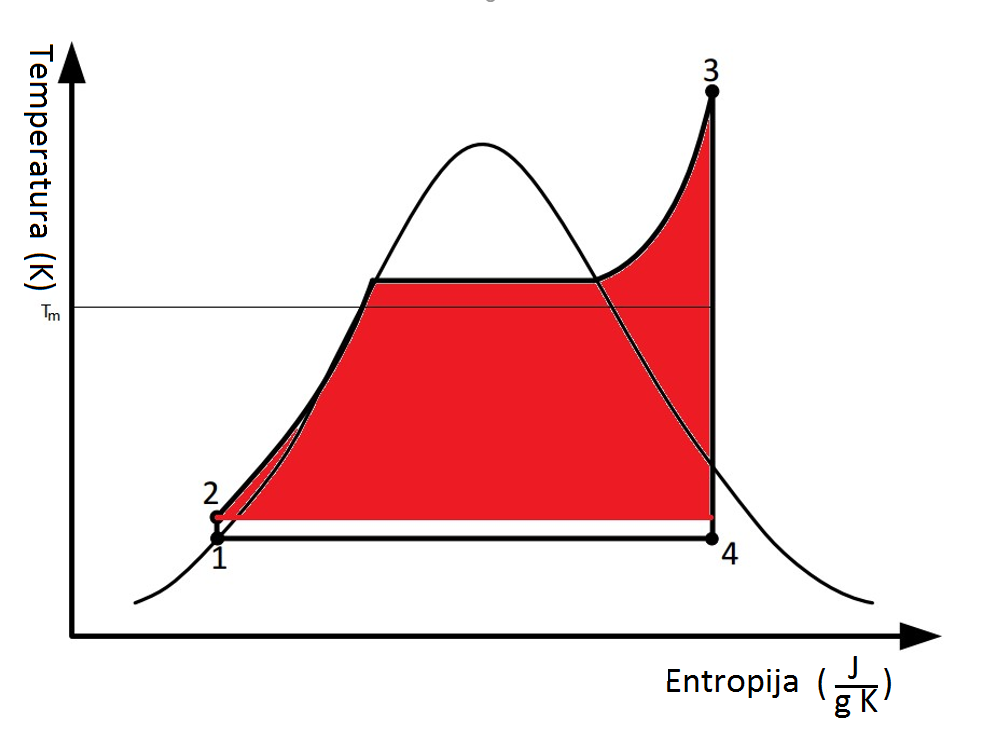
\includegraphics[width=0.95\columnwidth]{Untitled2.png}
	\captionof{figure}{Grafikon za predstavitev srednje temperature}
	\label{TS1}
\end{minipage}
Srednjo temperaturo izračunamo po enačbi \ref{eq14}
\begin{equation}
	T_m=\frac{h_3-h_2}{s_3-s_2}
	\label{eq14}
\end{equation}
\begin{minipage}{\linewidth}
	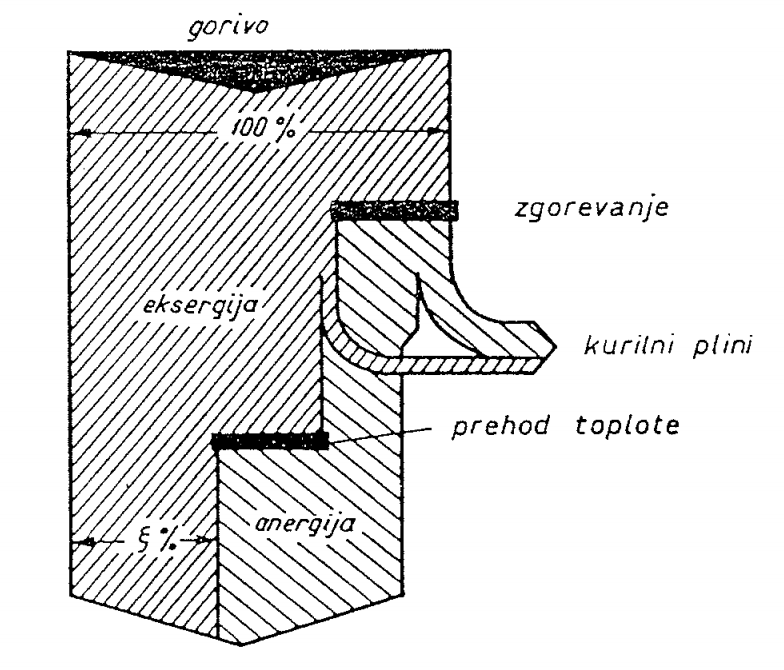
\includegraphics[width=\columnwidth]{Tokenergij.png}
	\captionof{figure}{Pretok energije v parnem kotlu\citep{Orel}}
	\label{kot2}
\end{minipage}
\subsection{Turbina}
Delovanje turbine vidimo na sliki \ref{TS} med točko 3 in 4. Izkoristek turbine lahko predstavimo v dveh delih, notranji in mehanski. Med seboj sta neodvisna.\citep{Katebi}
\begin{minipage}{\linewidth}
	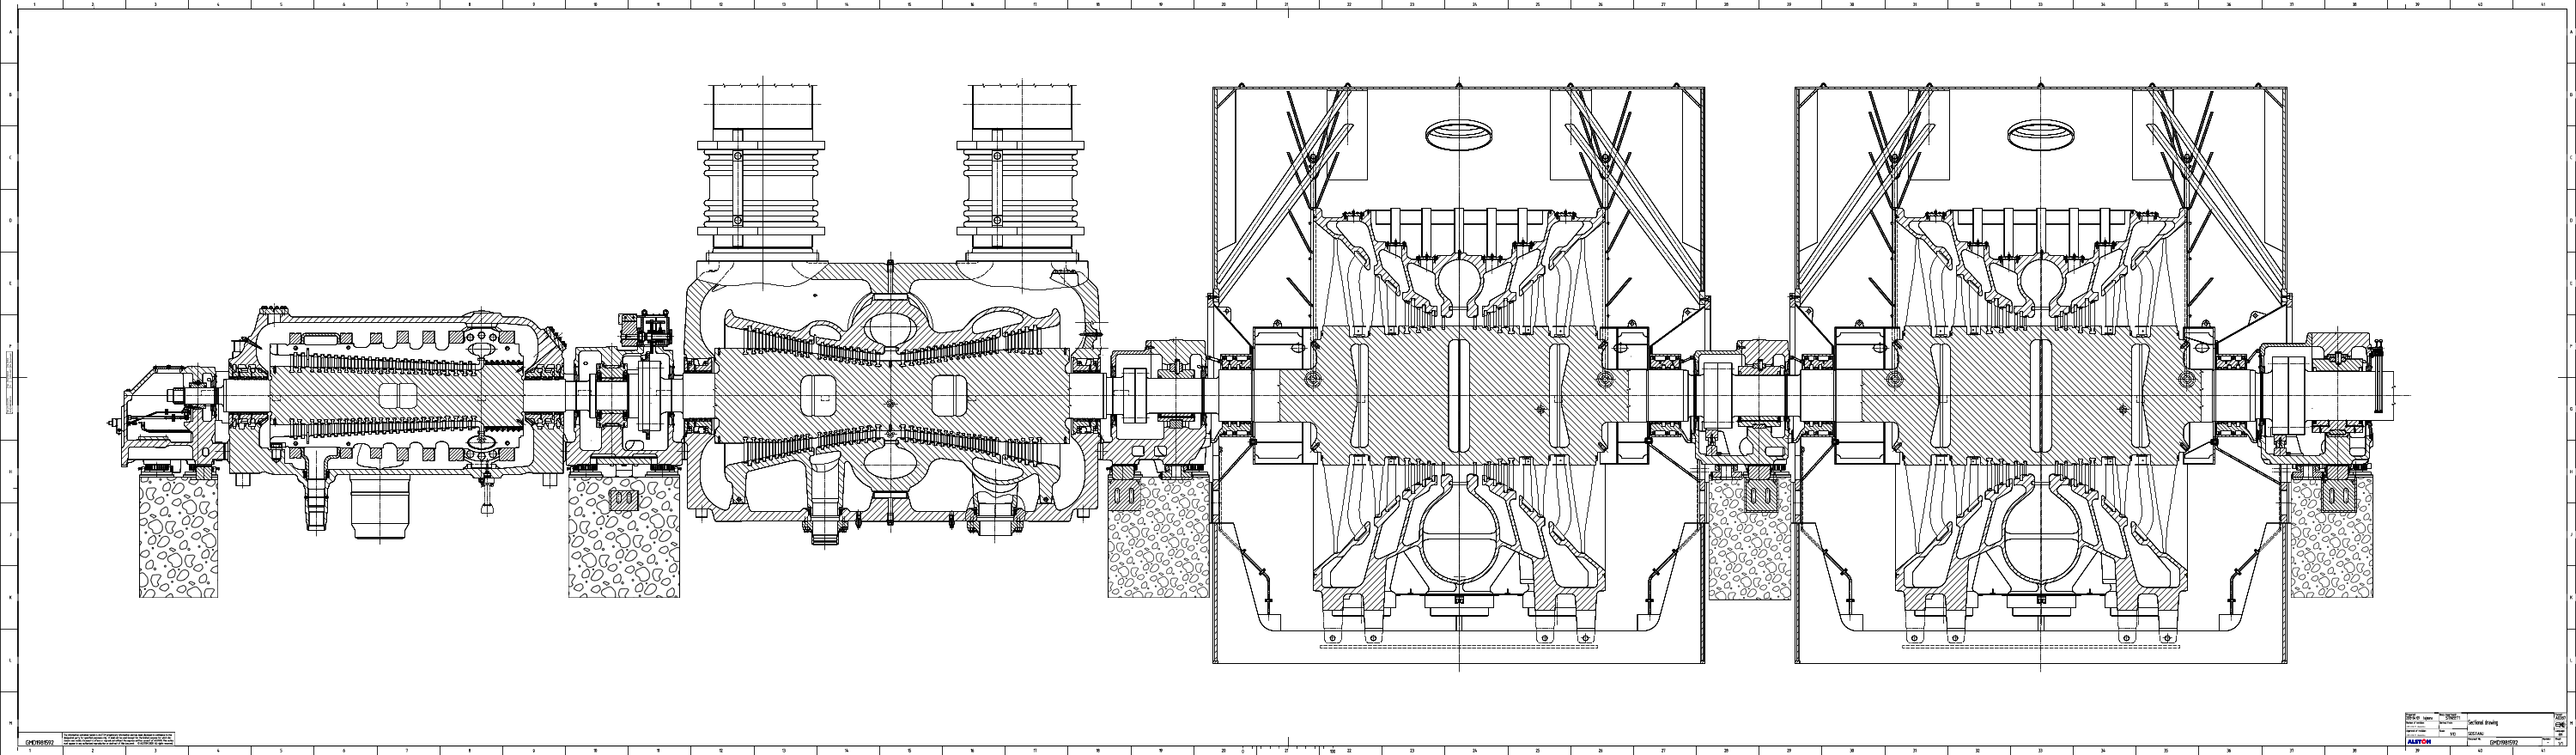
\includegraphics[width=\columnwidth]{prerez-turbina-bloka-6.png}
	\captionof{figure}{Turbina TE Šoštanj bloka 6 \citep{Sostanj}}
	\label{sostanj}
\end{minipage}
\subsubsection{Notranji izkoristek}
Toplotne ali notranje izgube predstavljajo izgube:
\begin{itemize}
	\item v šobah in vodilih lopatic 
	\item	v delovanju lopatic 
	\item	zaradi propuščana 
	\item	zaradi uhajanja toplote 

\end{itemize}
Vodna para je imela vrednost entalpije, kot je prikazano na sliki 1 v točki 3 na izstopu iz kotla. V cevovodu od parnega kotla do turbine, se para ohladi za temperaturo $\Delta T$ (na sliki \ref{TS} izgub v cevovodih ni prikazanih vendar so približno od 5 do $10^\circ \mathrm{C}$). Padec tlaka je odvisen od dolžine cevovoda, števila kolen, ventilov itd. Tlačne izgube so lahko tudi do 15 barov. 

Zaradi zmanjšanja zgoraj omenjenih veličin pare, je tudi entalpija pare manjša. Razpoložljiv padec na turbini je tako manjši od teoretičnega. Izgube se pojavijo tudi pri ekspanziji pare. To so izgube v šobah, trenju rotorja in ventilacije.  Notranji izkoristek turbine $\eta_{notr}$ je tako razmerje med teoretičnim toplotnim padcem $\Delta h$ in dejanskim $h_{dej}$. \citep{Orel}
\begin{equation}
	\eta_{notr}= \frac{h_{dej}}{\Delta h} =1- \frac{h_{izgub}}{\Delta h}
\end{equation}
\subsubsection{Mehanski izkoristek}
Mehanski izkoristek $\eta_{meh}$ je definiran kot razmerje moči na sklopki turbine $P_e$ in notranji moči turbine $P_i$.
\begin{equation}
	\eta_{meh}= \frac{P_e}{P_i}
\end{equation}
\subsection{Generator}
V TE se uporablja generator s cilindričnim rotorjem imenovan turbo generator. Izgube v generatorju se pojavijo zaradi trenja in ventilacije $P_{tr,vent}$. To so mehanske izgube. Imamo tudi električne, ki nastanejo zaradi izgub v železu $P_{Fe}$ in v bakru $P_{Cu}$. Izgube v železu se pojavijo zaradi histereze materiala. Izgube v bakru se pojavijo zaradi upornosti bakra. Izgube so pri velikih generatorjih tako velike, da je potrebno navitja hladiti (slika \ref{rot}). Izkoristek geneatorja  $\eta_{gen}$ je določen kot:
\begin{equation}
	\eta_{gen}=1- \frac{P_{Fe}+P_{Cu}+P_{tr,vent}}{P_{prej}}
\end{equation}
\begin{minipage}{\linewidth}
	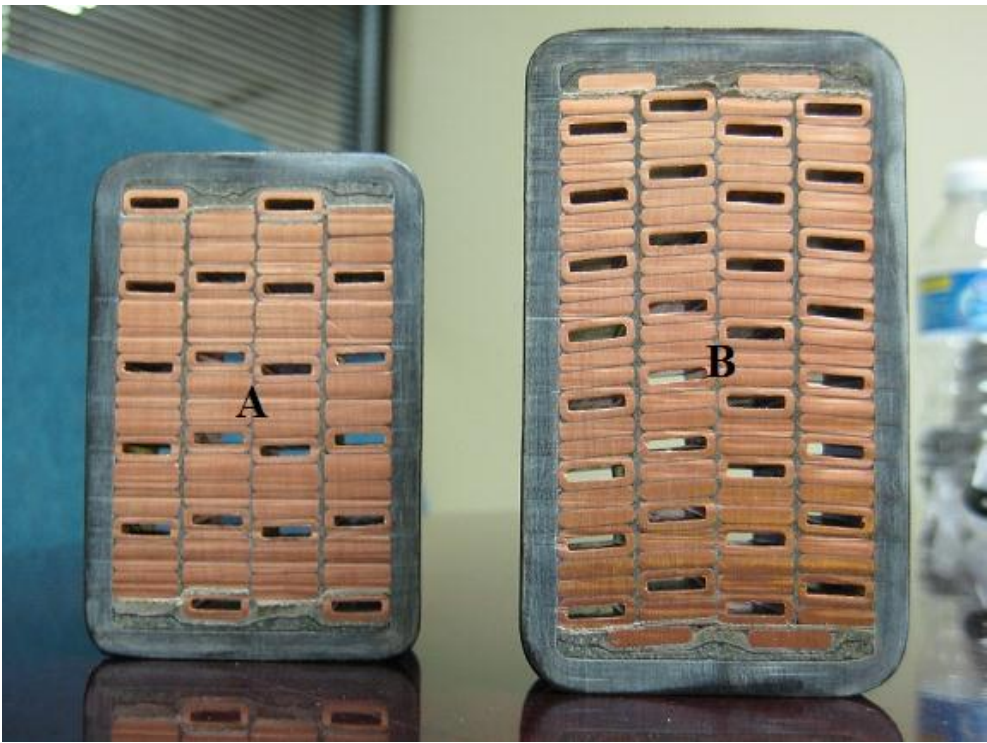
\includegraphics[width=0.95\columnwidth]{rotor.png}
	\captionof{figure}{V statorskem navitju je v nekaterih vodnikih prostor za dovod hladilne tekočine (vodik) \citep{Sostanj}}
	\label{rot}
\end{minipage}
\subsection{Lastna raba}
Vsaka elektrarna za svoje delovanje potrebuje elektriko. Ob zagonu TE morajo operaterji najprej zagreti kotel. Elektriko potrebujemo za delovanje črpalk, ki poganjajo vodo oz. paro po cevovodih. TE porabijo do 7\% proizvedene moči, kar lahko vključimo v skupni izkoristek. \citep{Tuma}
\begin{equation}
	\eta_{lr}=1-\frac{P_{lr}}{P_{gen}}
\end{equation}
$P_{lr}$ predstavlja moč lastne porabe, $P_{gen}$ pa proizvedeno električno moč generatorja.
\section{Rezultati pregleda literature}
Ob poznavanju izkoristkov posameznega dela TE, lahko izračunamo skupni izkoristek  $\eta_{TE}$.\citep{Gasperic}
\begin{equation}
	\eta_{TE}= \prod_i^n\eta_i=\eta_{kp}\eta_{"crp}\xi_k\eta_{not}\eta_{meh}\eta_{gen}\eta_{lr}
\end{equation}
\begin{minipage}{\linewidth}
	\captionof{table}{\emph{Razpon izkoristkov posameznega dela termoelektrarne.\citep{Tuma}}} 
	\label{tab:title}
	\begin{tabular}{  l c }
  		\hline
  		 \bf{Izkoristek} & \bf{Vrednost} \\
		\hline
		$\eta_{kp}$			&	0,48-0,65 	\\ \hline
		$\eta_{"crp}$ 		&	0,70-0,90	\\\hline
		$\eta_k	$			&	0,82-0,90	\\\hline
		$\xi_k	$			&	\~0,85	\\\hline
		$eta_{not}$			&	0,85-0,90	\\	\hline
		$\eta_{meh}$		&	0,95	\\\hline
		$\eta_{gen}$		&	0,96-0,98 (če jih hladimo z vodikom)\\
							&	 drugače 0,95-0,97 		\\\hline
		$\eta_{lr}$			&	0,92-0,97	\\\hline
		$\eta_{TE}$			&	0,35-0,44		\\\hline
  		\hline
	\end{tabular}
\end{minipage}
\vspace{5mm} % vertikalni razmak 5mm
\section{Razprava}
V tabeli 1 vidimo približne izkoristke, ki najbolj vplivajo na skupni izkoristek TE. Najbolj izstopa izkoristek krožnega procesa in ne kakšen poseben del TE.
Načrtovalci elektrarne so posamezne dele optimirali, pri krožnem procesu pa je kjučna termodinamika tekočin. Za boljši izkoristek bi morali  vodi odvzeti čim več entalpije (najbolje bi bilo entalpija v točki 3 na sliki 1 $h_3\rightarrow 0 \frac{\mathrm{J}}{\mathrm{g}}$. Z uporabo vode je to nemogoče doseči, saj voda pri 273 K pri normalnem zračnem tlaku, začne prehajati v trdo agregatno stanje.
\section{Zaključek}
Na končni rezultat najbolj vpliva termodinamika vode. Ljudje ponavadi poznajo samo podatek o skupnem izkoristku TE in mislijo, da se izgube pojavljajo predvsem pri sežigu. S tem delom sem opisal dele termoelektrarne in z njim predstavil ključni element, ki vpliva na skupni izkoristek. 
\small
\begin{thebibliography}{} 
\bibitem[1]{Gasperic}S. Gašperič, „Vaje za predmet Konvencionlani viri električne energije,“ v CIGRED, Portorož, 2015. 
\bibitem[2]{Orel}B. Orel, Energetski pretvorniki 2, Ljubljana: Univerza v ljubljani, 1993. 
\bibitem[3]{Katebi}S. G. Abokhatwa in R. Katebi, „Modeling and supervisory control design for combined cycle power plant,“ IEEE, p. 333, 2012. 
\bibitem[4]{Sostanj}„Termoelektrarna Šoštanj,“ 19 1 2016. [Elektronski]. Available: http://www.te-sostanj.si/si/proizvodnja/parne-turbine/turbina-bloka-6.
\bibitem[5]{Rotor}P. Habinac, „Menjava rotorja glavnega generatorja v NEK,“ Diplome mariborske univerze, Izv. 16, p. 5, 2012. 
\bibitem[6]{Tuma}M. Sekvačnik in M. Tuma, „Energetski sistemi- preskrba z električno energijo in toploto,“ Ventil, Izv. 16, pp. 55-58, 2004. 
\bibitem[7]{Wiki}„Wikipedia,“ 17 9 2014. [Elektronski]. Available: \ref{https://sl.wikipedia.org/wiki/Entalpija}. [Poskus dostopa 13 12 2016].
\end{thebibliography}
\normalsize
\end{multicols}
\end{document}